\documentclass[shortpaper]{revdetua}

\usepackage{scicite}
\usepackage{hyperref}

\usepackage{amsmath}
\usepackage{multicol}
\usepackage{setspace}

\usepackage{enumitem}

\usepackage{graphicx}
\usepackage{caption}
\usepackage{float}
\usepackage{subcaption}

\usepackage{verbatim}

\usepackage{booktabs}

\begin{document} %%%%%%%%%%%%%%%%%%%%%%%%%%%%%%%%%%%%%%%%%%%%%%%%%%%%%%%%%%%%%%%%%%%%%%%%%%%%%%%%%%%%%%%%%%%%%%%%%%%%%%%%%%%%%%%%%%%%%%%%%%%%%%%%%%%%%%%%%%%%%%%
 
\Header{2}{85122}{Dezembro}{2019}{1}

\title{
    \LARGE{{\bf Project 3: Frequent Items Counting \/}}
    \vspace{-20pt}
}

\author{
    \Large{{\bf A Study on Memory-Efficient Algorithms\/}}\\\\\\
    Filipe Pires [85122] \& João Alegria [85048]\\
    \\
    {\bf Advanced Algorithms\/}\\
    \normalsize{Department of Electronics, Telecommunications and Informatics}\\
    \normalsize{University of Aveiro}\\
} 

\maketitle %%%%%%%%%%%%%%%%%%%%%%%%%%%%%%%%%%%%%%%%%%%%%%%%%%%%%%%%%%%%%%%%%%%%%%%%%%%%%%%%%%%%%%%%%%%%%%%%%%%%%%%%%%%%%%%%%%%%%%%%%%%%%%%%%%%%%%%%%%%%%%%%%%%%%

\begin{abstract}
    Determining the most frequent items on a data stream has many applications and is a hot topic on the research community of the field.
    The challenges inherent of data stream processing in a memory efficient way are very much worth exploring and some of the existing solutions already provide
    with great optimization strategies.

    In this report, we focus on one of the most famous approximate counters to determine an estimation of the most frequent words of literary works from several 
    authors in several languages and compare it to an exact counter.
    We also present a few conclusions drawn from the study applied to the dataset.
\end{abstract}

\begin{keywords}
    Probabilistic Counter, Count-Min Sketch, Memory-Efficient Algorithms
\end{keywords}

\section{Problem Contextualization}\label{problem} %%%%%%%%%%%%%%%%%%%%%%%%%%%%%%%%%%%%%%%%%%%%%%%%%%%%%%%%%%%%%%%%%%%%%%%%%%%%%%%%%%%%%%%%%%%%%%%%%%%%%%%%%%%%%

When dealing with large datasets there are many operations that require the calculation of properties of each element. 
The presence of frequent events throughout the data might be a potential aspect worth exploring.
However, counting problems present obstacles when dealt with in very large contexts, and the difficulties are undoubtedly accentuated when the contexts morph 
into data streams.
As continuous sources of real time events, data streams present big challenges when processing each event in a precise and reliable way.
Many solutions have appeared throughout the years as means of dealing with these challenges by creating reliable approximations that, without using too many 
resources, still permit inferring the same conclusions that one is in search of.
These solutions are typically based on probabilistic approaches that do not compromise the results but add an error factor. 

The previous works of both authors of this paper address the application of approximate counters with fixed or descending probabilities of updating counts on 
the context of word counting in literary works \cite{alegria} \cite{filipe}.
This time, the same literary works will be used to estimate the most frequent words, with the text corpus considered as data streams with the help of a different 
and more complex strategy to reduce resource usage.
This report was written for the course of 'Advanced Algorithms', taught by professor Joaquim Madeira for the master's in Informatics Engineering at DETI UA and 
it describes the work done for the course's 3rd assignment \cite{trab3}. 
We chose the hypothesis "Hipótese A-2 – Contagem dos Itens Mais Frequentes" as we were interested in knowing how low could memory usage go without compromising
the outcome, i.e. how much memory could be saved while ensuring that the code still accomplished its purpose and returned approximations not too distant from 
the exact counters' values.

We create data streams to simulate a real world scenario and test the effectiveness and performance of the algorithm Count-Min Sketch.
Other available alternatives were: Frequent-Count, proposed by Misra \& Gries; Lossy-Count, by Manku \& Motwani; Space-Saving-Count, by Metwally.
We also discuss the differences and similarities between book translations.

\section{Dataset}\label{dataset} %%%%%%%%%%%%%%%%%%%%%%%%%%%%%%%%%%%%%%%%%%%%%%%%%%%%%%%%%%%%%%%%%%%%%%%%%%%%%%%%%%%%%%%%%%%%%%%%%%%%%%%%%%%%%%%%%%%%%%%%%%%%%%%

The dataset used, as already mentioned in chapter \ref{problem}, is based on literary works and in some of their translations. 
All of the books were obtained from \textit{Project Gutenberg}\cite{gutenberg}. 
The chosen books and respective languages are presented below:

\setlist{nolistsep}
\begin{itemize}
    \item \textit{Alice in the Wonderland}, by Lewis Carol - written in English, German, French and Italian
    \item \textit{A Christmas Carol}, by Charles Dickens - written in English, Finnish, German, Dutch and French
    \item \textit{King Solomon's Mines}, by H. Rider Haggard - written in English, Finnish and Portuguese
    \item \textit{Oliver Twist}, by Charles Dickens - written in English, French and German
    \item \textit{The Adventures of Tom Sawyer}, by Mark Twain - written in English, Finnish, German and Catalan 
\end{itemize}

Since provident from the \textit{Project Gutenberg}, the books come with headers and annotations that identify authors, sources and additional metadata that 
was not relevant for our study; with this in mind, we preprocessed the various book files to remove the metadata that could cause unwanted variation on results. 
This process was quite simple and was only necessary the usage of a text editor and the manipulation of some regular expressions. 

\section{Frequent Word Identification}\label{algs} %%%%%%%%%%%%%%%%%%%%%%%%%%%%%%%%%%%%%%%%%%%%%%%%%%%%%%%%%%%%%%%%%%%%%%%%%%%%%%%%%%%%%%%%%%%%%%%%%%%%%%%%%%%%%

Identifying the most frequent words in a text stream was achieved using two very different strategies.
On the first one, the program keeps record of all words that appear in the information stream along with an exact count of each word - this allows it to 
determine at any time which words are the most frequent.
The second, on the other hand, is a far more memory-friendly solution that uses hash functions to avoid storing the pair $(word, counter)$.
In this chapter we discuss the implementation of both solutions for the use case of identifying the most frequent words on literary works.

\subsection{Exact Counter}

The exact counter is the gold standard when creating alternative solutions that save time, memory or other resource at the cost of precision.
It is by the values computed by it that the other counters are evaluated.

Its implementation consists of a regular dictionary of words as keys and counts as values, constantly updated as new words appear on the text stream.
There are conditions, however, to update this dictionary.
The incoming word must contain at least two characters and cannot belong to a list of stop-words defined \textit{a priori}.
This is done to prevent considering words that are irrelevant, i.e. do not offer any practical value to the study such as articles or prepositions.

Stop-words are managed by an external library \cite{stop-words}, capable of dealing with all languages of our dataset. 

\subsection{Count-Min Sketch}

The Count–Min Sketch (CM Sketch) is a probabilistic data structure that serves as a frequency table of events in a data stream.
This means it works essentially like Bloom-Filters (BFs).
However, they are used differently and therefore sized differently: 
a CM Sketch typically has less entries than the total number of different events (or words in our case) of the stream, related to the desired approximation 
quality, while a counting BF is sized to match the total number of different events. 

The solution uses hash functions to map word occurrences to frequencies, but saves memory space at the expense of over-counting some words due to collisions.
The effect of these phenomena is addressed ahead.
\newline

The implementation of our CM Sketch was taken from the resources made available by the course's professor.
As it served perfectly for our purposes, we found it unreasonable to reach our own implementation at the risk of adding imperfections that could compromise our study.
Nevertheless, we offer a description of how it works and how we introduced it to the use case.

If the same conditions defined in the Exact Counter are verified for the current word on the text stream, the word is passed to the \textit{update()} method of 
the \texttt{CountMinSketch} class.
This method then applies all its hash functions to the word and increments the values on the hash tables on the respective entries.

As the word counts either have the exact count or suffer from over-counting, the value considered as more trustworthy is the one whose result from hashing and 
updating returned the smallest value - the one with less occurrences of collisions - (hence the name count-MIN sketch).
It is this value that is returned when the class instance is queried.

\texttt{CountMinSketch} receives two regulatory parameters that allow us to control the overestimation factor.
These are \texttt{m}, the size of the hash tables, and \texttt{d}, the number of hash tables.
The first regulates how significant is the overestimation since only the smallest value is returned by \textit{query()} so the more tables there are, the 
smallest will be the difference between the real count and the one returned.
The second reduces the probability of collisions since more hash tables means more complex hashes less likely to be equal.
Two alternative parameters could have been used, \texttt{delta} and \texttt{epsilon}, that regulate the probability of query error and the query error factor 
and internally define \texttt{m} and \texttt{d} but in our case we sticked with the first two.

\section{Literary Study} %%%%%%%%%%%%%%%%%%%%%%%%%%%%%%%%%%%%%%%%%%%%%%%%%%%%%%%%%%%%%%%%%%%%%%%%%%%%%%%%%%%%%%%%%%%%%%%%%%%%%%%%%%%%%%%%%%%%%%%%%%%%%%%%%%%%%%%

As a form of automation and to enable us to quickly study the behavior of the chosen algorithm, we created a script in Python that allows us to change some of 
the necessary parameters and run the solution for a given input stream in a straightforward, command-based manner.
The signature of our script is as follows:

\vspace{-5pt}
\begin{center}
    \begin{verbatim}
    python3 frequentWordFinder.py [-h]
    [-o outputFolder] [-d numHash] 
    [-m numColumns] <inputFolder>
    \end{verbatim}
\end{center}
\vspace{-15pt}

The \textit{outputFolder} is a parameter that indicates the folder where the resulting files should be stored (the default folder is called "out" and is 
generated if it does not exist), \textit{numHash} and \textit{numColumns} correspond to the number of hashes and the number of columns the user wants to be used 
when creating the \texttt{CountMinSketch}, explained in chapter\ref{algs}; these 3 parameters are optional and they all have default values 
(outputFolder:"out", numHash:1000, numColumns:5).
The \textit{inputFolder} is a mandatory parameter since it's the folder where the source data should be present; this data is assumed to be preprocessed, 
since that will generate the best results, without any noise form the headers and annotations mentioned in chapter \ref{dataset}.
\newline

What we did to study the performance of CM Sketch was to record its results for various inputs and parameter combinations and resort to data visualization tools 
to understand its behavior.
The tested inputs were all of the literary works from our dataset, and the tested parameters were combinations of \texttt{numColumns} within the range [200,4000] 
and \texttt{numHash} within the range [1,10].

\begin{equation}
    E_{r} = \frac{E}{X} \times 100
    \label{eq:1}
\end{equation}

\newpage
The exact count is considered to compute both the error of the approximate count and its relative error.
The error ($E$) of an estimation for a word is defined as the difference between its exact count ($X$) in the text stream and the count given by the Sketch.
The relative error ($E_r$) corresponds to error percentage given by equation \ref{eq:1}.







\section{Results \& Discussion} %%%%%%%%%%%%%%%%%%%%%%%%%%%%%%%%%%%%%%%%%%%%%%%%%%%%%%%%%%%%%%%%%%%%%%%%%%%%%%%%%%%%%%%%%%%%%%%%%%%%%%%%%%%%%%%%%%%%%%%%%%%%%%%%

Lorem ipsum ...

% \begin{table}[h!]
% \centering
% \begin{tabular}{@{}c|ccc@{}}
% \toprule
%                       & \textbf{EC} & \textbf{ACFP} & \textbf{ACLP} \\ \midrule
% \textbf{All Words}    & 5116614     & 4886294       & 4797502 \\
% \textbf{Top 10 Words} & 40899       & 22916         & 6635    \\ \bottomrule
% \end{tabular}
% \caption{Number of bytes used in the counter values.}
% \end{table}
% \vspace{-12pt}

% \vspace{-10pt}
% \captionsetup[figure]{labelformat=empty}
% \begin{figure}[H]
%     \centering
%     \setlength{\belowcaptionskip}{-12pt}
%     \includegraphics[width=\linewidth]{wordCount_ACC_DU.png}
%     \caption{Fig. 1: Counter estimations for the top 10 words.} 
%     \label{fig:1}
% \end{figure}

%%%%%%%%%%%%%%%%%%%%%%%%%%%%%%%%%%%%%%%%%%%%%%%%%%%%%%%%%%%%%%%%%%%%%%%%%%%%%%%%

\section{Conclusion}

Lorem ipsum ...

%%%%%%%%%%%%%%%%%%%%%%%%%%%%%%%%%%%%%%%%%%%%%%%%%%%%%%%%%%%%%%%%%%%%%%%%%%%%%%%%

\bibliography{report.bib} 

\newpage
\textbf{ }
\newpage
\appendix

\begin{figure*}[]
    \begin{subfigure}[t]{0.5\textwidth}
        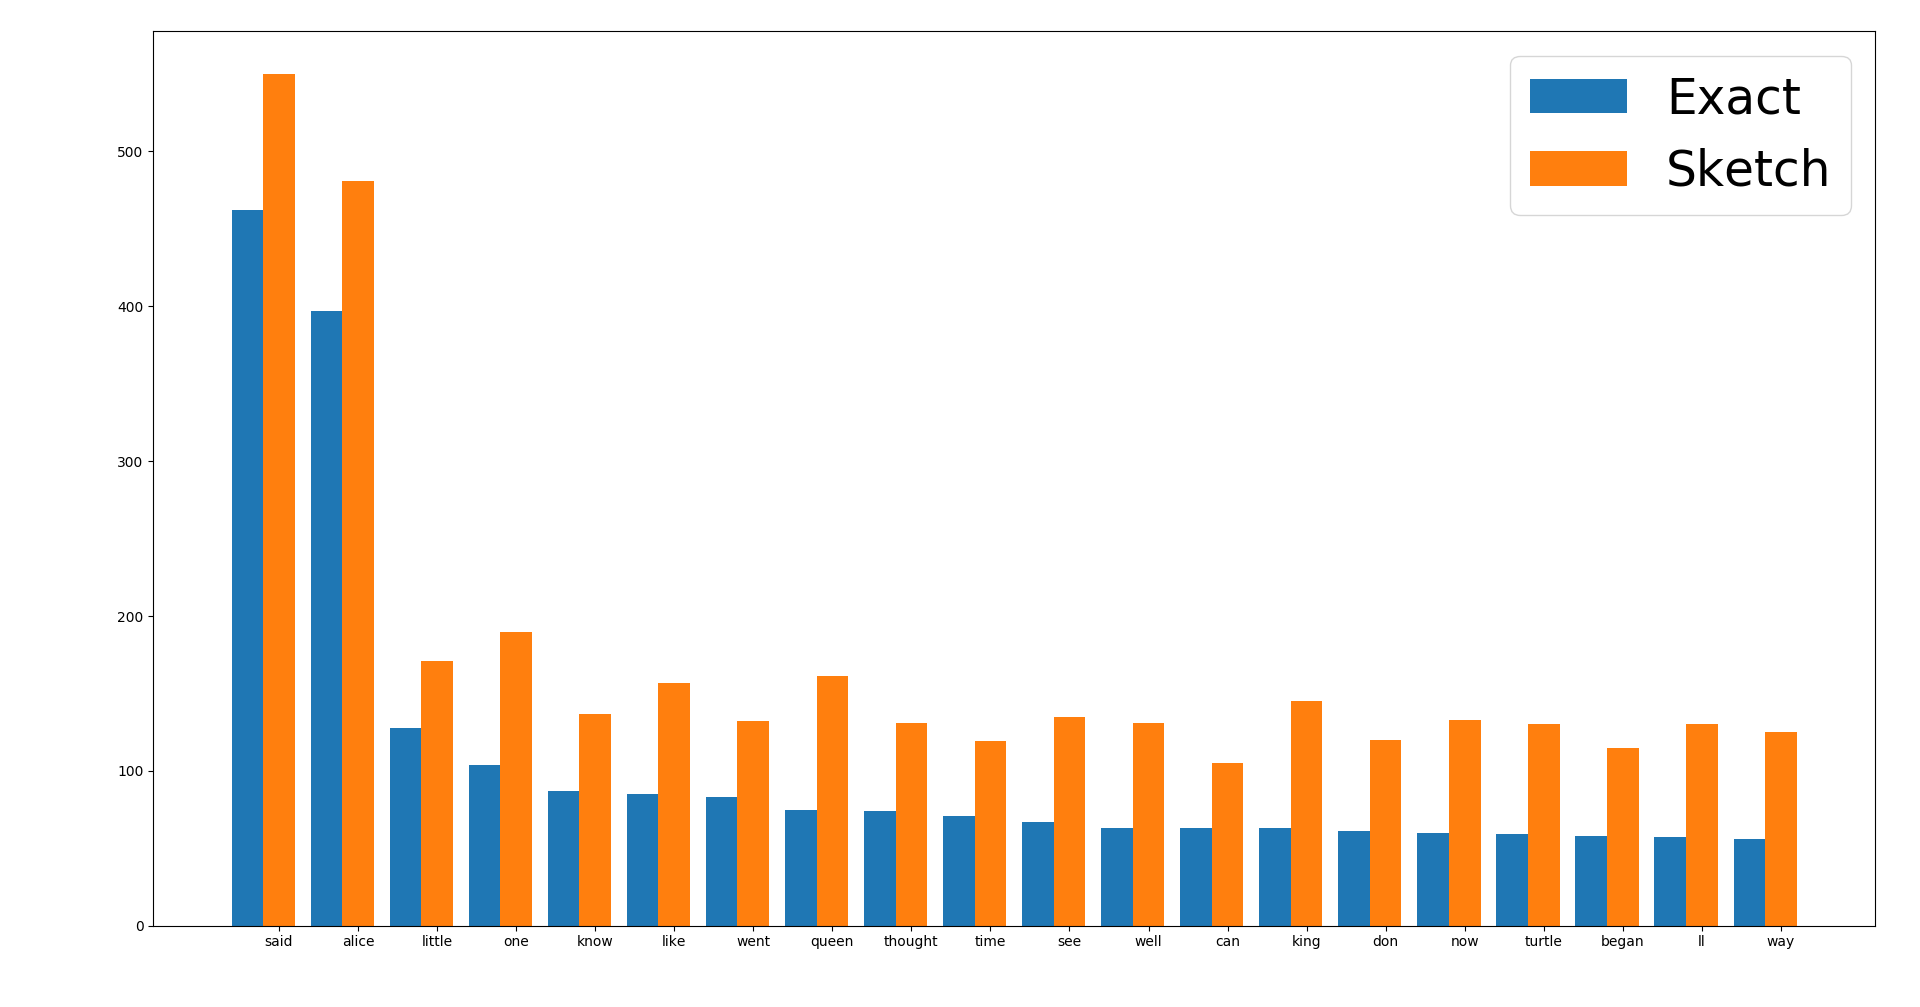
\includegraphics[height=1.6in]{englishAlice100_5.png}
        \caption{Lorem ipsum}
    \end{subfigure}
    \begin{subfigure}[t]{0.5\textwidth}
        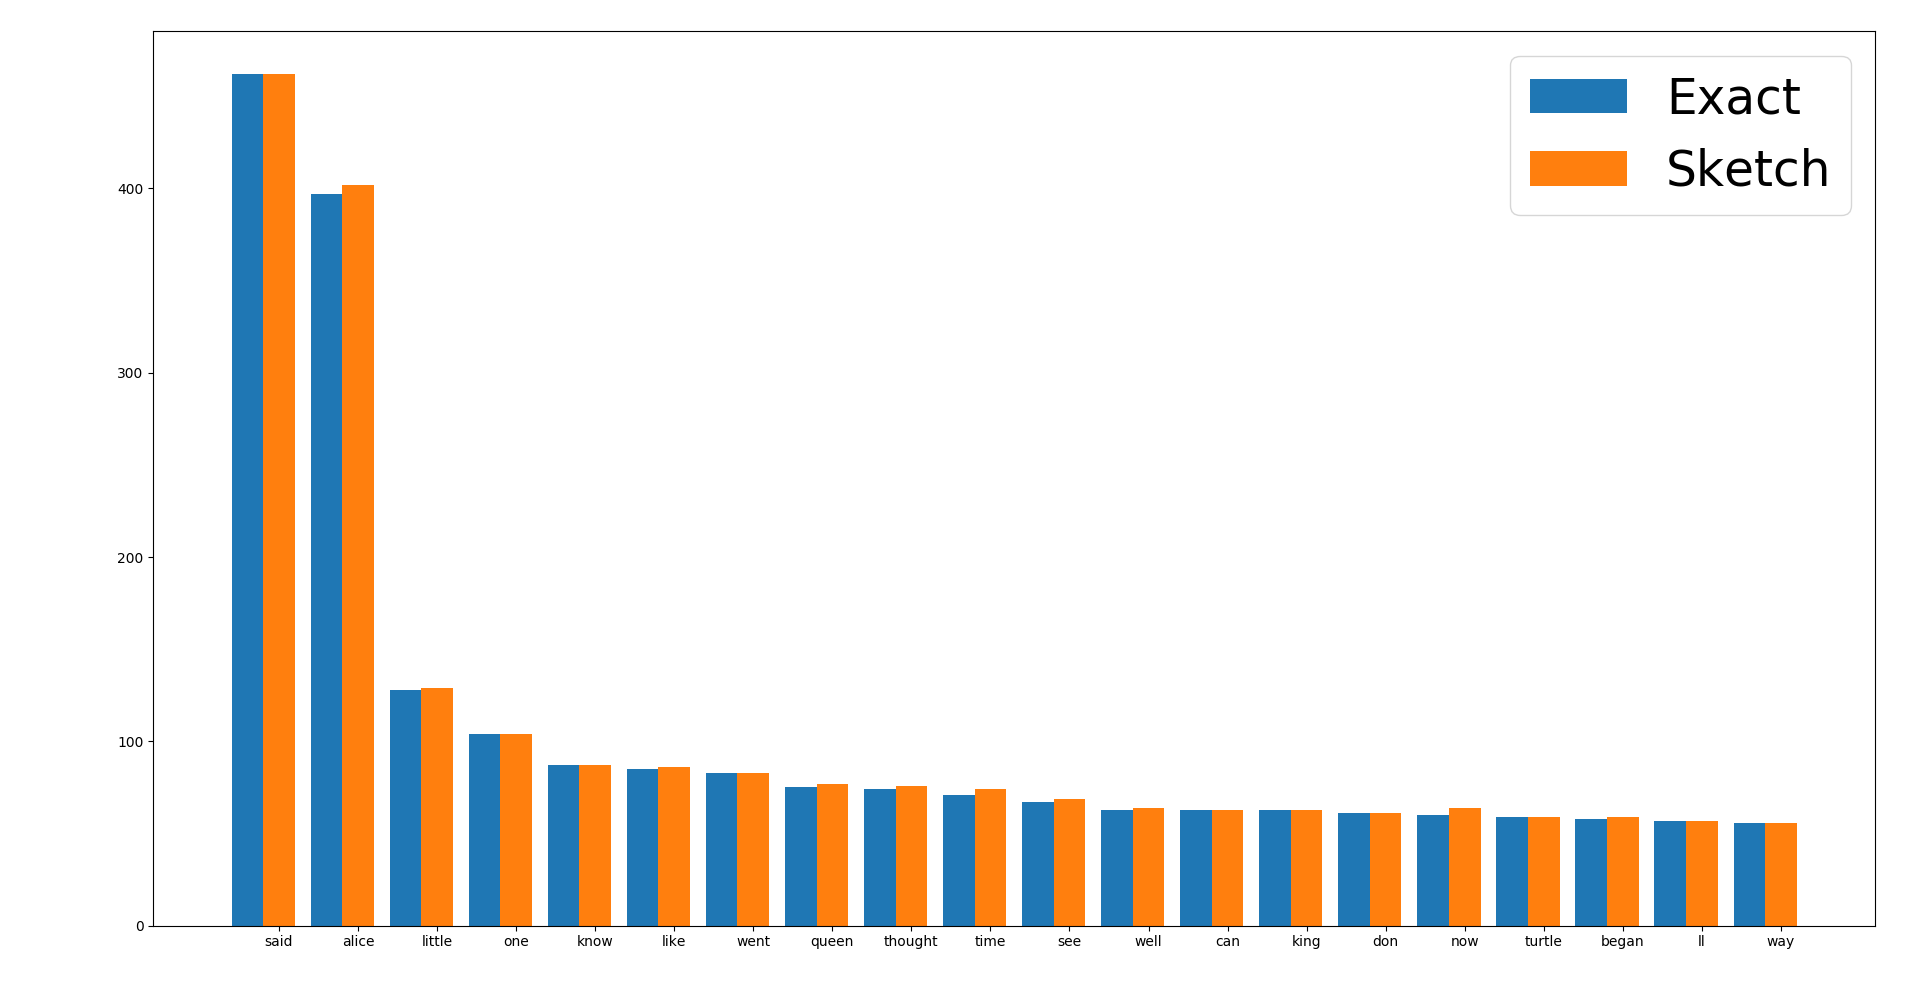
\includegraphics[height=1.6in]{englishAlice1000_5.png}
        \caption{Lorem ipsum}
    \end{subfigure}
    \begin{subfigure}[t]{0.5\textwidth}
        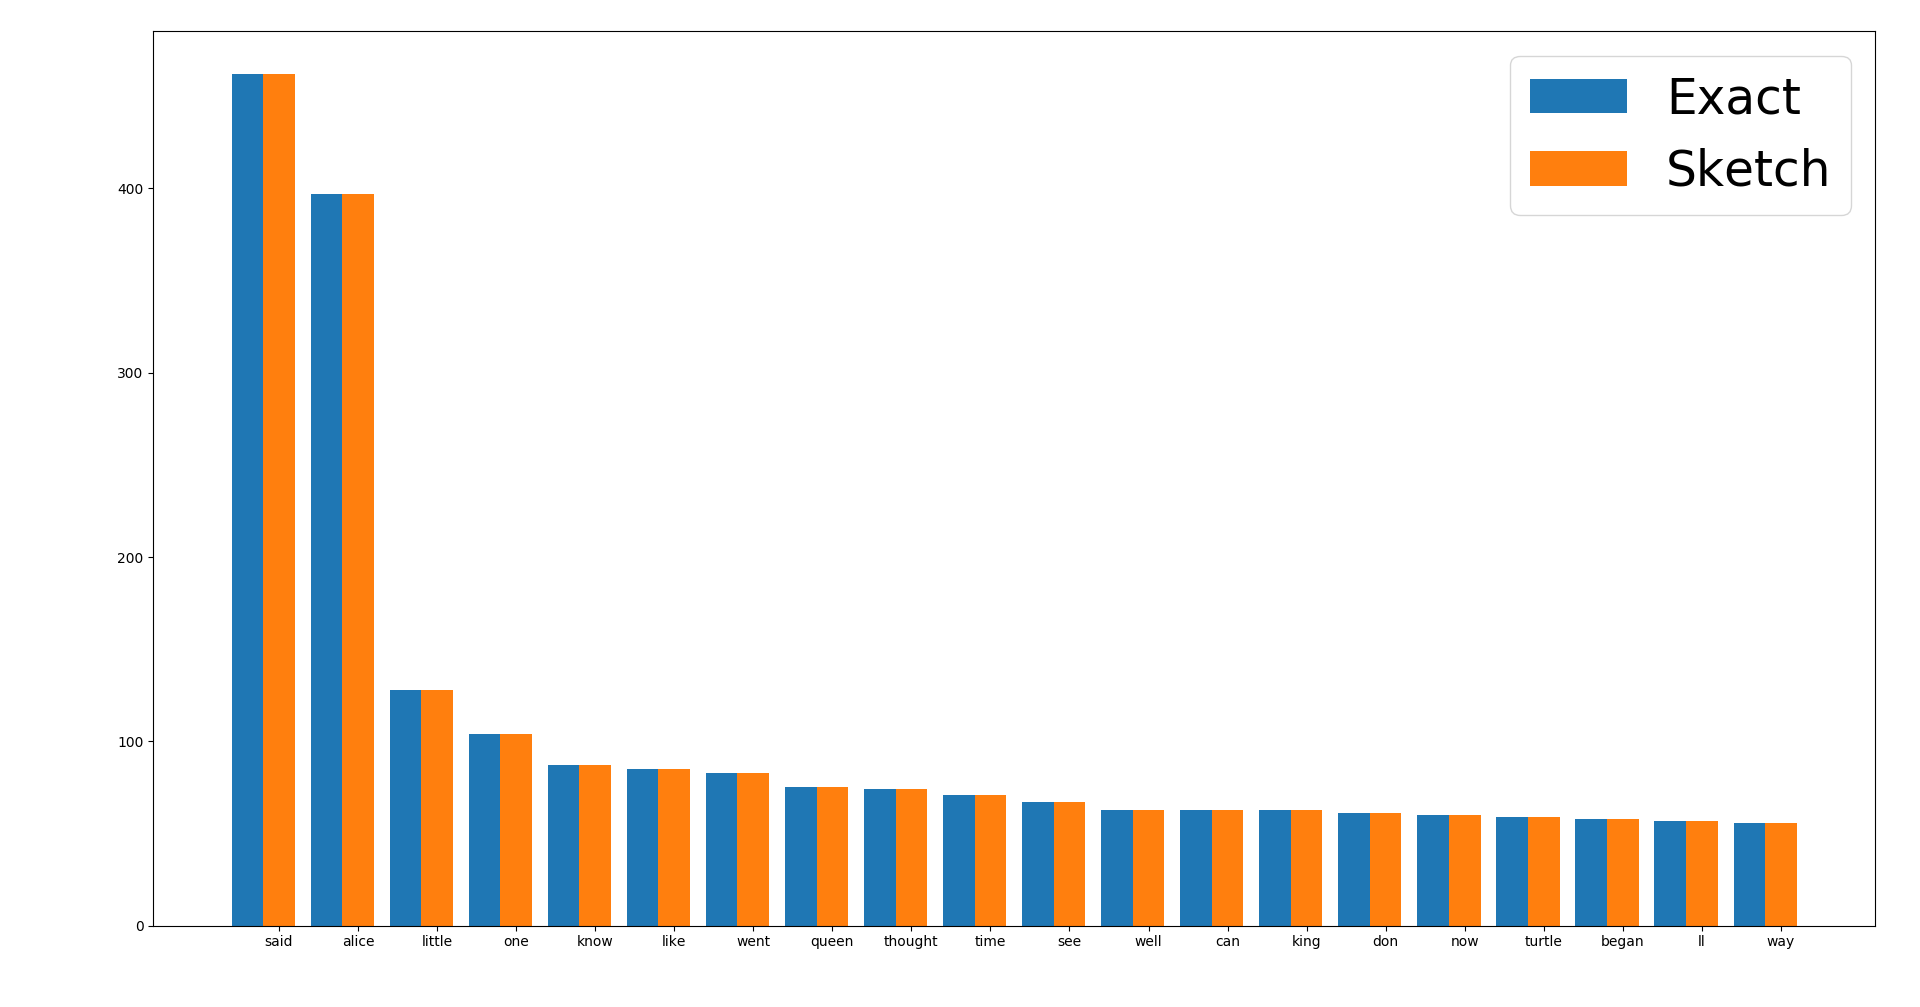
\includegraphics[height=1.6in]{englishAlice10000_5.png}
        \caption{Lorem ipsum}
    \end{subfigure}
    \begin{subfigure}[t]{0.5\textwidth}
        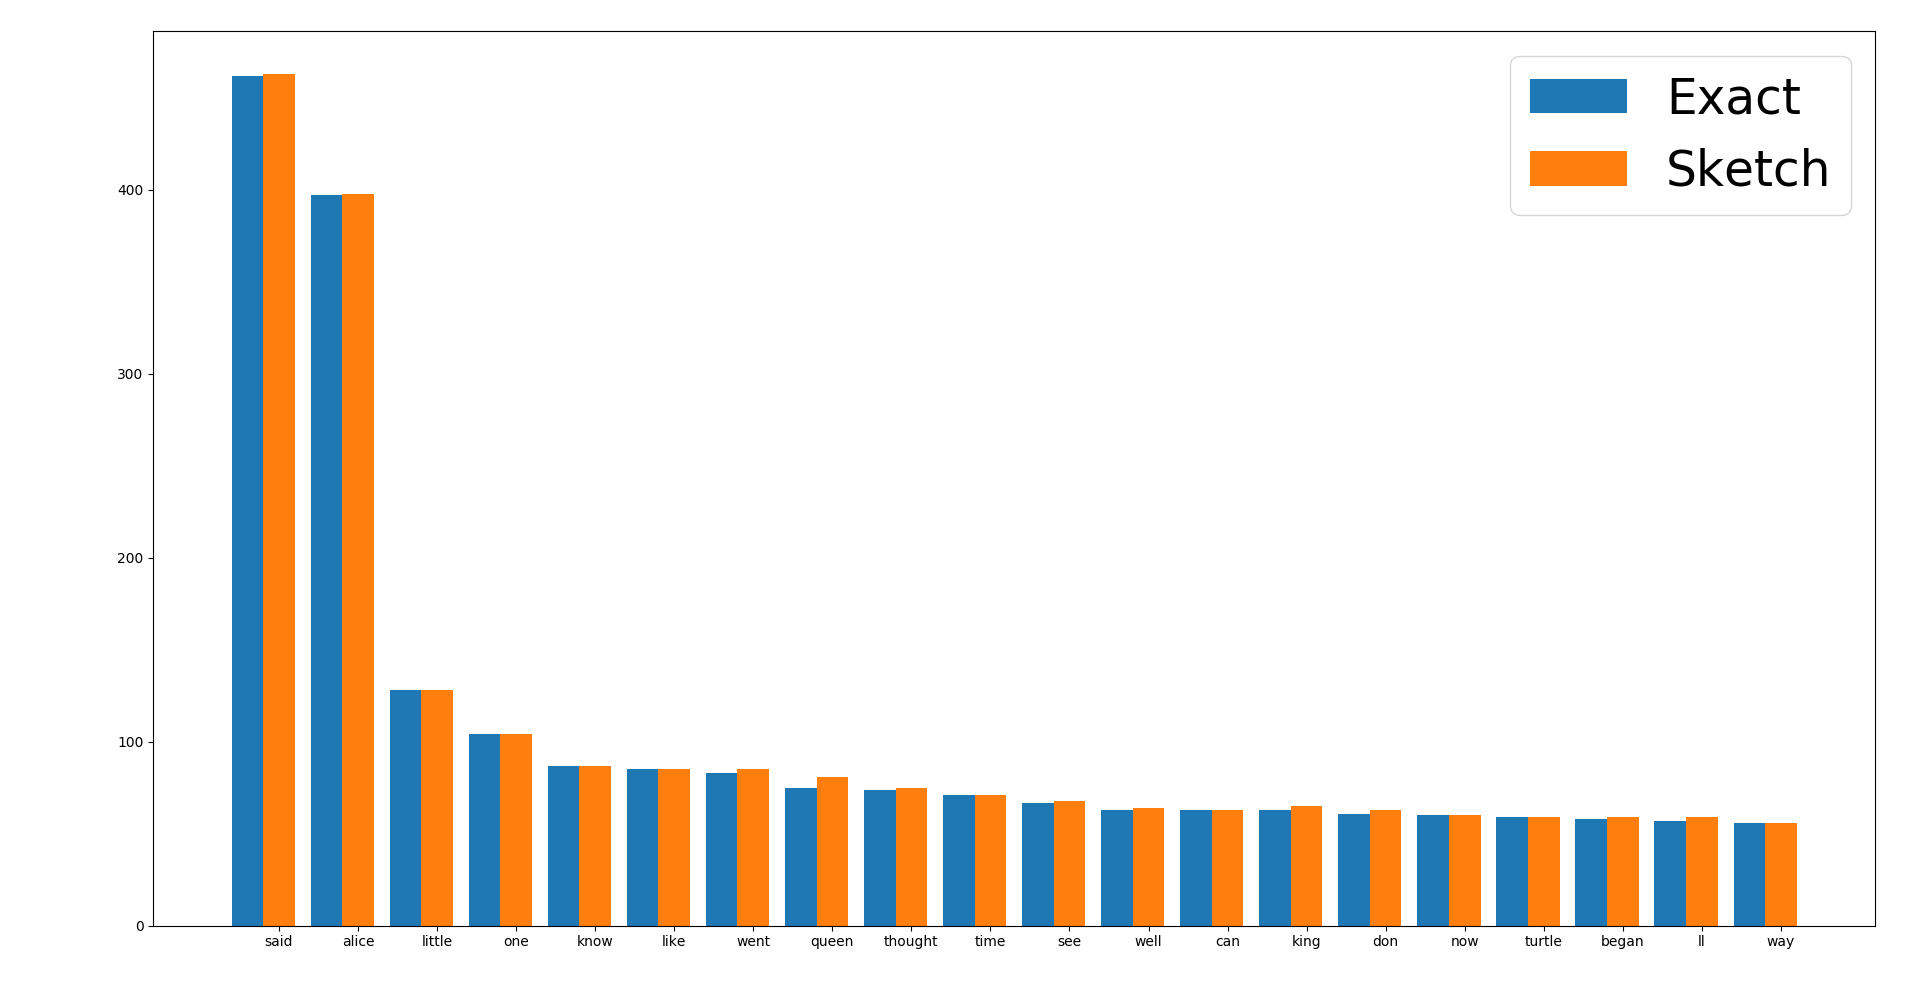
\includegraphics[height=1.6in]{englishAlice1000_6.png}
        \caption{Lorem ipsum}
    \end{subfigure}
    \begin{subfigure}[t]{0.5\textwidth}
        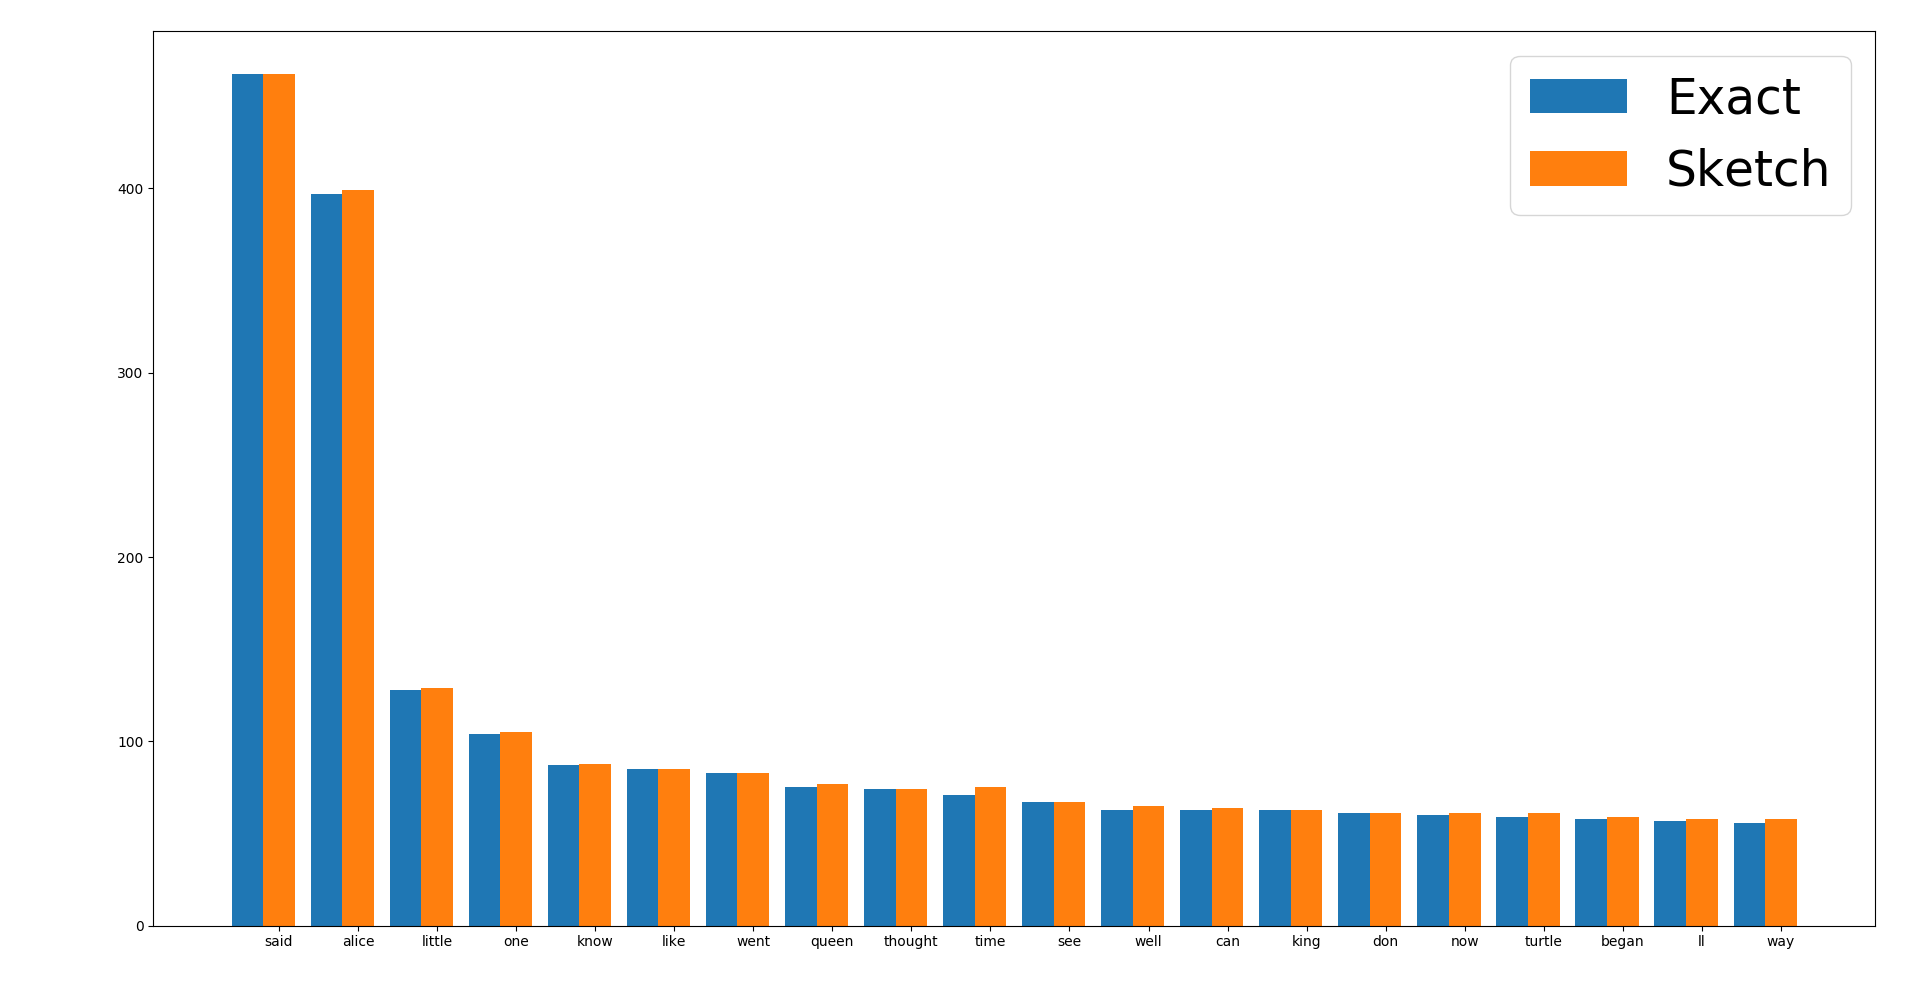
\includegraphics[height=1.6in]{englishAlice1000_8.png}
        \caption{Lorem ipsum}
    \end{subfigure}
    \begin{subfigure}[t]{0.5\textwidth}
        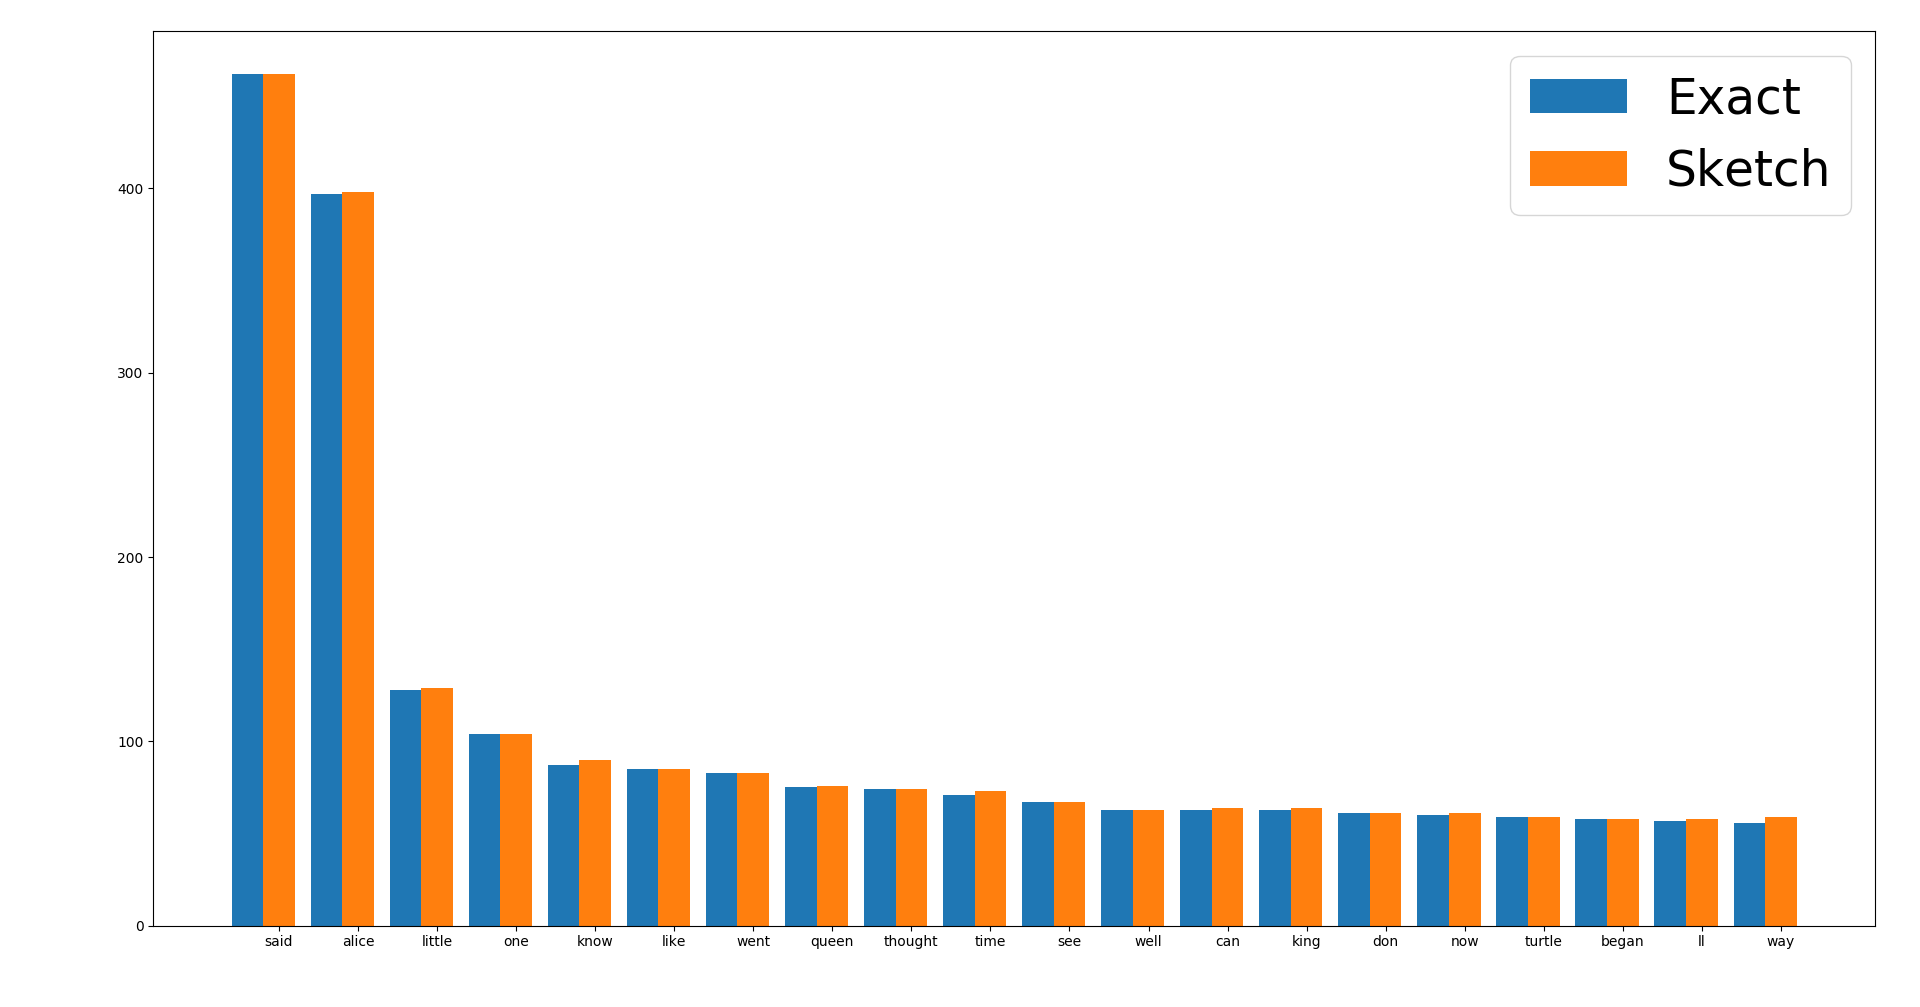
\includegraphics[height=1.6in]{englishAlice1000_10.png}
        \caption{Lorem ipsum}
    \end{subfigure}
    \caption{Caption place holder}
\end{figure*}

\end{document}
